\documentclass{beamer}
\usetheme{metropolis}
\usepackage{pgfpages}
\usepackage{listings}
\usepackage{csquotes}
\usepackage{hyperref}

\setbeameroption{show notes on second screen}

\title{Agile Development}
\subtitle{Tools for moving fast and not breaking things}
\author{Kevin Wang \and Aidan Wolk}
\year=2020\relax
\month=01\relax
\day=23\relax
\date{\today}
\institute{DevX}
\logo{
\includegraphics[height=0.5cm]{assets/devxlogo.png}}

\makeatletter
\def\beamer@framenotesbegin{
  % at beginning of slide
  \usebeamercolor[fg]{normal text}
  \gdef\beamer@noteitems{}
  \gdef\beamer@notes{}
}
\makeatother

\begin{document}

\maketitle

\section{Introduction}

\subsection{Who are we}

\begin{frame}{whoami}
  \begin{columns}
    \begin{column}{0.48\textwidth}
      \textbf{\Large Kevin Wang}

      \begin{description}
        \item[LA Hacks] Tech Director Emeritus
        \item[DevX] Tech Advisor
      \end{description}

      \texttt{\tiny github: @xorkevin}
    \end{column}
    \begin{column}{0.48\textwidth}
      \textbf{\Large Aidan Wolk}

      \begin{description}
        \item[Broomie] Engineering Manager
        \item[DevX] Tech Advisor
      \end{description}

      \texttt{\tiny github: @awolk}
    \end{column}
  \end{columns}
\end{frame}
\note[itemize]{
  \item We are not experts
  \item But we are passionate about developer experience
  \item And want to share our perspectives from our experiences building,
    deploying, and maintaining applications
  \item As your tech advisors, come to us with questions, we are happy to help
}

\subsection{Motivation for this talk}

\begin{frame}{Why is the dev process important?}
  \begin{displayquote}[Anonymous][.]
    A good craftsman never blames his tools
  \end{displayquote}

  A corollary:

  \begin{displayquote}[][.]
    A good craftsman should know his tools
  \end{displayquote}
\end{frame}
\note[itemize]{
  \item Often, developers are focused on new frameworks, languages, etc., but
    not enough thought is given to the dev process
  \item An old adage states that a good craftsman should never blame his tools
  \item Therefore, a good craftsman should know his tools
  \item Working on a tech project is more than just knowing a technology or a
    framework
  \item It involves knowing how to integrate your work with the ecosystem
    around it
  \item Thus, you need to know your tools, their capabilities, and their
    limitations
}

\begin{frame}{Brief Overview}
  \begin{itemize}
    \item Version Control
      \begin{itemize}
        \item Git
        \item Best practices
      \end{itemize}
    \item Containerization
      \begin{itemize}
        \item Docker
        \item How to begin using it
      \end{itemize}
  \end{itemize}
\end{frame}
\note[itemize]{
  \item You have probably heard of these tools before
  \item If not, do not worry, that is what this talk is for
  \item We want to focus on best practices for using these tools and how you
    can incorporate them into your project
}

\section{Version Control}

\subsection{What is it}

\begin{frame}{Version Control}
  \begin{itemize}
    \item History tracking for files
    \item Changes can be committed and tracked by the VCS
    \item Modern VCS's can easily merge changesets
      \begin{itemize}
        \item as you will need for your projects
      \end{itemize}
  \end{itemize}
\end{frame}
\note[itemize]{
  \item History tracking is important for projects
    \begin{itemize}
      \item Viewing a subset of changes allows you to easily locate bugs
        instead of having to search the entire project
    \end{itemize}
  \item Storing history allows you to share those changes with others
    \begin{itemize}
      \item Allows multiple people to work on the same project
    \end{itemize}
  \item Every project should be using version control
}

\begin{frame}{How did we get here?}
  \begin{description}
    \item[SCCS] Bell Labs, 1972, early software VCS
    \item[RCS] Purdue, 1982, delta storage
    \item[CVS] University Amsterdam, 1986, multi-user
    \item[SVN] CollabNet, 2000, spiritual successor of CVS
    \item[Git] Linus Torvalds, 2005, distributed VCS
  \end{description}
\end{frame}
\note[itemize]{
  \item Common complaint is that VCS are complex and unintuitive
    \begin{itemize}
      \item Can be helpful to look at history, to give context, and understand
        why these complexities were introduced
    \end{itemize}
  \item Source code control system, one of the first software VCS, major
    upgrade over punch cards, kept track of single files, single user
  \item Revision control sytem, tracked diffs between versions
  \item Concurrent versions system, developed for MINIX development, can work
    across the network, centralized development
  \item Subversion, spiritual successor of CVS
  \item Git, developed to maintain Linux development to address scalability
}

\subsection{Git}

\begin{frame}{Why Git?}
  \begin{center}
    
\includegraphics[height=0.75cm]{assets/gitlogo.png}
  \end{center}
  \begin{itemize}
    \item Distributed version control system
      \begin{itemize}
        \item Multiple independent branches across computers
        \item No branch is inherently “more important” than the other
      \end{itemize}
    \item High industry adoption
    \item Most popular source code repository hosting services e.g. GitHub,
      GitLab use Git
    \item \href{https://www.youtube.com/watch?v=4XpnKHJAok8}{Youtube - Tech
      Talk: Linus Torvalds on git}
  \end{itemize}
\end{frame}
\note[itemize]{
  \item DVCS is designed to allow many people to work on the same project at
    the same time
  \item In a centralized VCS, there is only one copy of the project, and all
    your changes are immediately made available to others
  \item Hence only a few people can work on the same file at the same time
  \item DVCS addresses this by having multiple copies of a project at the same
    time
  \item People can work on features independently of one another
  \item Git makes merging easy
  \item We highly encourage you to use Git
}

\section{Git}

\subsection{Conceptual overview}

\begin{frame}{Distributed VCS}
  \begin{center}
    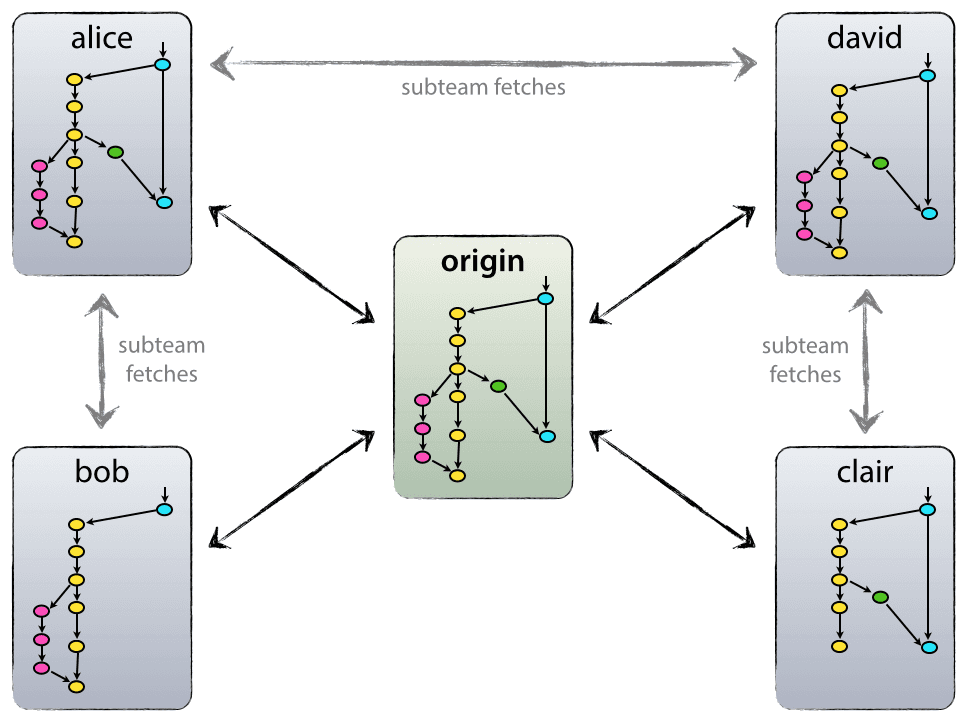
\includegraphics[width=\textwidth]{assets/gitdistributed.png}
  \end{center}
\end{frame}
\note[itemize]{
  \item Understanding Git conceptually is important to gain an intuition of
    what the commands do, and when to use them
  \item A Git repository is a set of files and their history of changes
  \item Everyone has their own copy of the repository that they can clone to
    work off of
  \item In practice, one of these copies of the repo will be designated the
    central source of truth copy, typically called origin and hosted at an
    easily accessible location like GitHub or GitLab, and it will serve as the
    method to send changes between team members
}

\begin{frame}{Commit graph}
  \begin{center}
    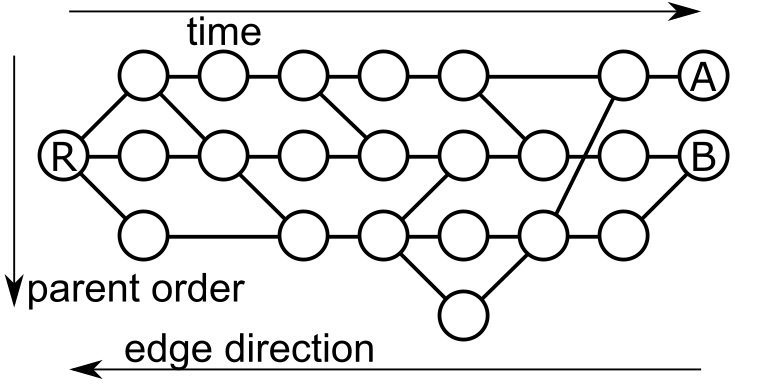
\includegraphics[width=\textwidth]{assets/gitgraph.png}
  \end{center}
\end{frame}
\note[itemize]{
  \item Changes in Git are organized in the form of commits
  \item A commit is conceptually a set of changed lines from an earlier commit
  \item These commits form a directed acyclic graph which encompass all the
    changes which have been committed to a repository
  \item Important to note that in a DVCS, the commit graph is not linear;
    changes can occur at the same time
}

\begin{frame}{Workflow}
  \begin{center}
    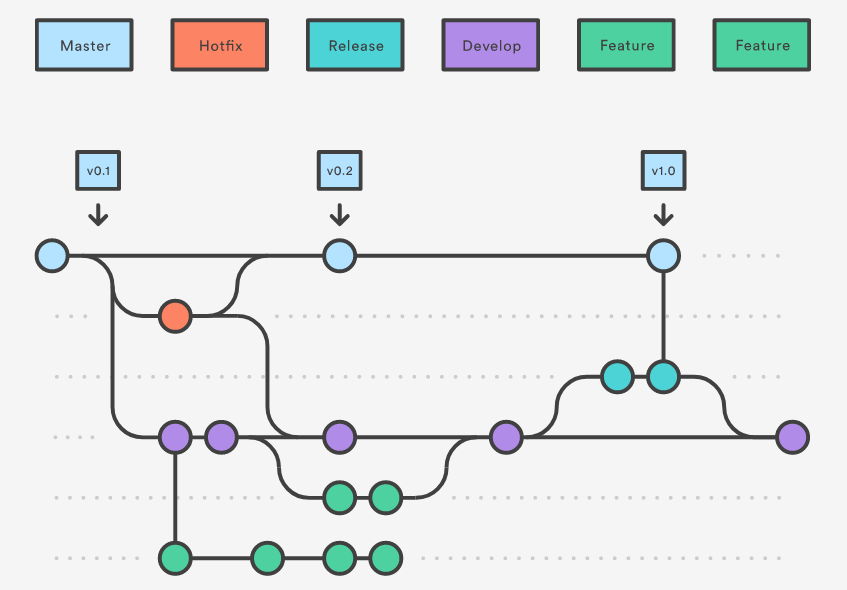
\includegraphics[width=\textwidth]{assets/gitworkflow.png}
  \end{center}
\end{frame}
\note[itemize]{
  \item Git is quite flexible and has features to support many workflows
  \item Branch is a label given to a particular path of commits
  \item Some teams prefer more trunk based development, where everyone commits
    to the same upstream origin branch, typically called master
    \begin{itemize}
      \item usually for small projects
    \end{itemize}
  \item Larger projects need a more scalable way to manage changes
  \item Typically will have a production, development, and feature branches
  \item Team members will work on their own features and merge them into the
    development branch when they are finished
  \item Use a flow that works best for you
}

\begin{frame}{Git}
  \Huge Demo
\end{frame}
\note[itemize]{
  \item basic git flow, add, commit, push
  \item clone, branch, pr flow
  \item pr review merge flow
}

\subsection{Best practices}

\begin{frame}{.gitignore}
  \begin{itemize}
    \item Only source code should be checked in
      \begin{itemize}
        \item Do \textbf{not} commit build artifacts to your repo
      \end{itemize}
    \item When X is reproducible from Y, X does not need to be checked in 99\%
      of the time.
      \begin{itemize}
        \item e.g. \texttt{node\_modules/} is reproducible from
          \texttt{package-lock.json}
      \end{itemize}
  \end{itemize}
\end{frame}
\note[itemize]{
  \item Too often I see \texttt{.DS\_Store} or \texttt{\_\_MACOSX} committed
  \item Those files should be ignored in your personal global
    \texttt{.gitignore}
}

\begin{frame}{More helpful Git}
  \begin{itemize}
    \item Commit \textbf{early} and \textbf{often}.
    \item PRs should be \textbf{short} and \textbf{atomic}.
    \item Use branch protection on GitHub.
    \item Rebase with care.
    \item \texttt{git diff} to view the changes between two commits.
    \item Some less frequently used commands:
      \begin{itemize}
        \item \texttt{git bisect}
        \item \texttt{git apply}, \texttt{git cherry-pick}
        \item \texttt{git blame}
      \end{itemize}
  \end{itemize}
\end{frame}
\note[itemize]{
  \item Commits should be thought of as an atomic unit of work.
  \item The longer a PR, the more difficult it is to review.
  \item PRs should not introduce partial functionality that breaks live
    features.
  \item Branch protection allows you to enable rules such as requiring PRs to
    be reviewed, and preventing direct merges to master.
  \item Feel free to rebase your own work that you have locally. But, do
    \textbf{not} rebase public history. Doing so will rewrite history for
    others, and Git will not be able to help you merge changes.
  \item Git provides many helpful commands to manage your work, and work with
    others
  \item One can better leverage these tools by adhering to good conventions
}

\section{Containerization}

\subsection{What is it}

\begin{frame}{Containerization}
  \begin{itemize}
    \item The definitive way to deploy and manage workloads at scale
    \item Modern container systems leverage cgroups in the Linux kernel
    \item Containers provide a virtualized OS to a process
      \begin{itemize}
        \item Distinct from a VM which provides virtualized hardware
      \end{itemize}
  \end{itemize}
\end{frame}
\note[itemize]{
  \item Containers provide a way to isolate processes based on CPU, memory,
    disk, network, etc.
  \item Containers were developed to manage workloads at scale, however, the
    virtualized OS interface gives developers other benefits as well
    \begin{itemize}
      \item Easy development environment setup
      \item Testing in environment before staging or production
      \item No more it works on my machine
      \item Easy process supervision
    \end{itemize}
}

\begin{frame}{Brief history}
  \begin{description}
    \item[Cgroups] Google, 2006, Linux kernel feature to provide processes
      isolation
    \item[Mesos] Berkeley, 2009, distributed process manager
    \item[Docker] 2013, both a container image format and runtime/engine
    \item[Kubernetes] 2014, distributed container orchestration system
  \end{description}
\end{frame}
\note[itemize]{
  \item Cgroups isolate processes based on CPU, memory, disk, network, etc.
  \item Mesos is a process manager for computer clusters, leverages cgroups
  \item Docker is containerization for the masses with a toolchain for easily
    creating and running containers
  \item Kubernetes is a distributed container orchestration system with a
    highly available, centralized scheduler
}

\subsection{Docker}

\begin{frame}{Why Docker?}
  \begin{center}
    
\includegraphics[height=0.75cm]{assets/dockerlogo.png}
  \end{center}
  \begin{itemize}
    \item Easy to work with containerization technology with wide support from
      various platforms and tools
    \item Toolchain includes everything from image creation to running
      containers
  \end{itemize}
\end{frame}

\section{Docker}

\subsection{Conceptual Overview}

\begin{frame}{Containers}
  \begin{center}
    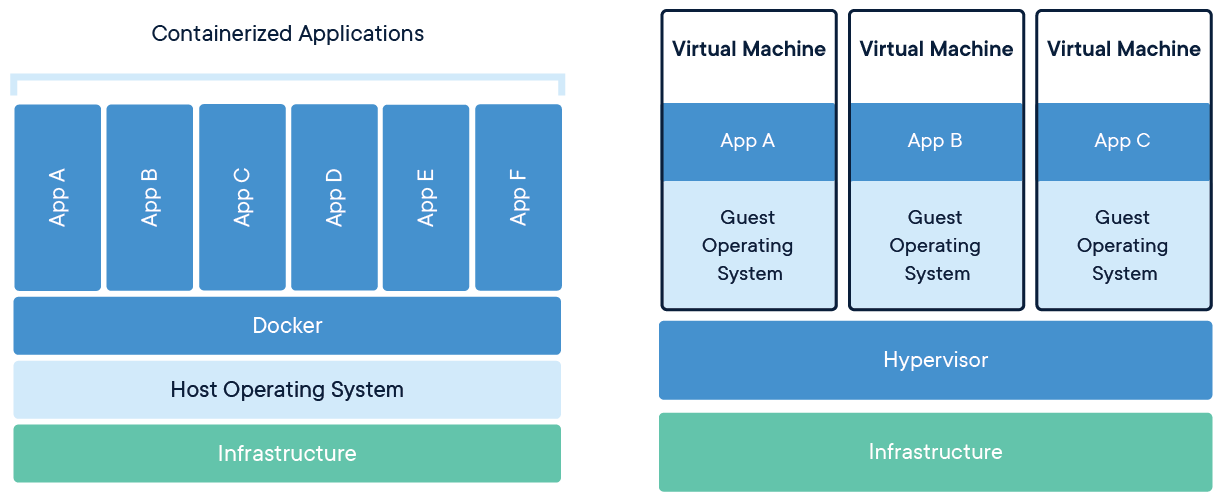
\includegraphics[width=\textwidth]{assets/dockercontainer.png}
  \end{center}
\end{frame}
\note[itemize]{
  \item Again, understanding the concepts behind Docker is an important
    prerequisite to using the tool
  \item This is the common image used to explain containers
  \item Containers are isolated processes that are presented a virtualized view
    of the OS
  \item Again, this is distinct from VMs which are operating systems which are
    presented a virtualized view of the hardware
  \item Containers are far lighter as they do not run an OS per app
}

\begin{frame}{Workflow}
  \begin{center}
    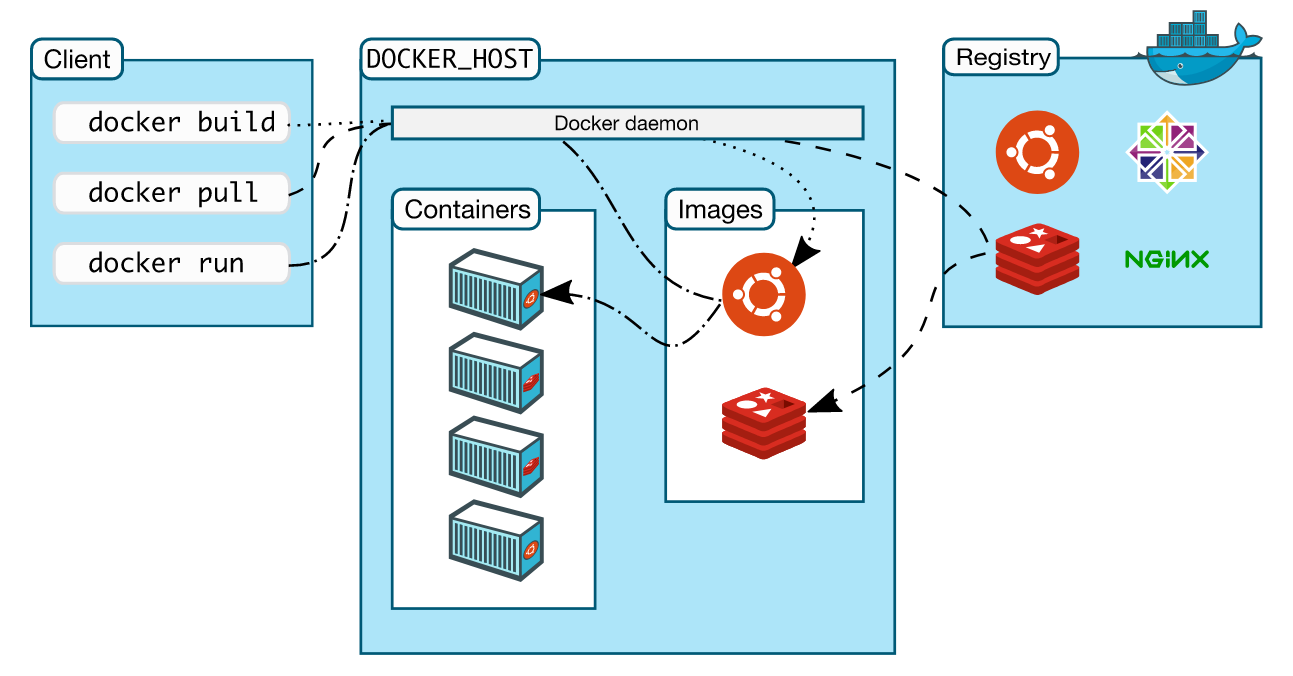
\includegraphics[width=\textwidth]{assets/dockerworkflow.png}
  \end{center}
\end{frame}
\note[itemize]{
  \item Docker has a daemon which manages the building of images, and the
    running of containers on a machine
  \item Images are a blueprint of how to create a container
  \item Containers are a running instance of an image
  \item Images can be named, tagged by version, and published on Docker
    registries
  \item If you want a private registry, look into ECR, the self-hosted
    \texttt{registry}, etc.
}

\begin{frame}{Docker}
  \Huge DEMO
\end{frame}
\note[itemize]{
  \item docker pull, docker run, psql into postgres
    \begin{itemize}
      \item expose port
      \item volume for persistent data
    \end{itemize}
  \item Dockerfile example packaging a Node app
  \item docker-compose and docker-compose.yaml example
}

\subsection{Best practices}

\begin{frame}{Helpful Docker}
  \begin{itemize}
    \item Docker containers are ephemeral
      \begin{itemize}
        \item Docker containers are stateless (aside from volumes)
        \item Do not expect data to persist by default
      \end{itemize}
    \item Infrastructure as code
      \begin{itemize}
        \item Docker is a large part of the IaC equation
        \item Treating your platform and infra as something that can fail
          allows you to be more resilient
        \item Redeploys should take seconds of human interaction rather than
          hours
      \end{itemize}
  \end{itemize}
\end{frame}
\note[itemize]{
  \item Again, Docker will help you the more you adhere to its conventions
}

\end{document}
